\chapter{Related Work}\label{cap:relatedWork}

In this chapter, some considerations on issues related to this work will be briefly presented, providing the reader with a comparative analysis between the current theme and other related areas and solutions. 

In the section \ref{sec:smartFactories}, the concept of "Smart Factories" will be addressed, including the origin of this topic, the advances made in the area, and the challenges faced. It will explore how the implementation of advanced technologies has revolutionized the industry, offering new opportunities and requiring adaptation by companies.

In Section \ref{sec:digitalTwin}, the state of the art in the realm of Digital Twin technology is explored, a field that has been gaining traction in recent years. The symbiotic relation of Digital Twin with contemporary industries is scrutinized, emphasizing how this technological paradigm facilitates a more comprehensive and immersive perspective for businesses by enabling simulations and virtual analyses of processes and products.

In Section \ref{section: woodFurnitureIndustryTraceabilityReview}, a broad introduction to various aspects of current traceability methodologies used in inventory and process control is presented. Particular attention is given to technologies such as QR Codes and RFID, which play significant roles in modern tracking systems and  more related to the work developed here..

Section \ref{section:stateOfArt} delves into the state of the art of traceability systems in the wood industry. It is noteworthy that there is a scarcity of published literature concerning this topic. Hence, a motivating factor for the publication of this work is to stimulate and contribute to the scientific discourse in this domain.

By analyzing these related topics, it will be possible to obtain a more comprehensive and grounded view on the innovations and trends that have impacted the industry, setting the stage for understanding the contributions and relevance of this work.


\section{Smart Factories}
\label{sec:smartFactories}

German experts have formed the concept of Industry 4.0 to promote a new industrial revolution\cite{Grabowska+2020+90+96}. This approach aims to promote a new generation of manufacturing facilities that use advanced technologies to optimize manufacturing and process control in real time. Countries in the European Union have adopted this model to improve the use of natural resources and increase the competitiveness of their industries, especially in view of the gradual transfer of their industrial leadership to emerging countries.

The "Smart Factory" concept started in industrialized regions. European countries were pioneers in developing this new concept of industry, especially Germany, which coined the term \emph{Industrie 4.0} in 2011 \cite{Grabowska+2020+90+96}. In recent years, the fall of competitiveness in the industrial sector of these countries due to low birth rates or high wages, made them adopt an industrial strategy led by the use of technologies such as robots, sensors, Big Data, machine learning, deep learning, \acrfull{iiot}, \acrfull{ai}, data analysis and telecommunication networks among devices \cite{HerreroMeasuringTheEffectivenessOfIndustrialProcesses}. For this reason, these regions recognized the potential of increased industrial automation as a means to address the shortage of skilled workers and to mitigate the impact of rising production costs on workers' salaries.

This new paradigm of industrialization is becoming increasingly important for companies in recent years. According to \textcite{Grabowska+2020+90+96}, it is expected that the implementation of modern technologies and new management techniques in line with Industry 4.0 will take over most manufacturing processes in the coming years. The use of \acrshort{ai} is part of these new gimmicks that have gained ground in the industry recently. In \textcite{PeresIASmartFactory} the topics involving \emph{deep learning} related to the industrial environment that recently showed the most research interest were: energy optimization, predictive maintenance and quality control. In addition, there have been major advances in process automation involving decision making, operations supervision, maintenance services, and safety systems \cite{KUMAR2022121284}. Thus, the innovations provided by a more technology-driven industry are becoming increasingly important as they make it possible to improve efficiency, reduce waste and errors, and increase productivity.

This new form of industrialization brings new features to the production chain. For example, the deepening of the digitalization of the industry beyond management. With the creation of "smart products". These are products that are integrated in the value chain and are part of the company's virtual environment. This approach facilitates p localization of the items on the factory floor, enables tracking of their progress throughout different stages of the production process, and allows for seamless communication of this information to customers regarding the status of their orders.\cite{economies6030046}.

Another important key point that this technology bring to the table is the possibility to help  corporations to improve the experience in the manufacturing of the product.  The use of an IIoT system allows an improved experience both for the consumer and for the product development team. From the end user's point of view, M2M communication can allow the customer to track the development status of the customized product in real time. This can be done by collecting data about the production process and making that data available to the customer through a portal or app. This can give the customer a clearer view of the progress of their order and increase satisfaction with the service. From the product development team's point of view, M2M communication can allow professionals to quickly obtain information about previous products with similar characteristics to the product being developed. This can be done by collecting attributes such as geometric information, material, lead time, etc. This can help the team to better understand customer needs and preferences and speed up the modeling process by reusing old designs.

\emph{"Smart factories"} is not a futuristic concept \textcite{Gilchrist2016}  \textcite{Gilchrist2016}. This form of vision is present in the form of production today and in past decades. For example, manufacturing a car involves the welding of parts, which can be done by \emph{"smart machines"} that are programmed to perform this work with precision. However, while one specific process is common to many different models of cars, other processes tend to be different in order to characterize one product as being distinct from another. In this production model, car parts can be moved to different parts of the factory and tracked to get their proper customizations. This greater production malleability allows a single production line to be able to produce products with different aspects.

The industry 4.0 present a greater flexibility among its processes due to the possibility of a interaction between cybernetic and physical systems \cite{Gilchrist2016}. In Industry 3.0, it is common to use \acrfull{erp} to plan the execution of manufacturing processes, besides the use of a software system commonly called \acrfull{mes}, which plays the role of managing the execution of previously planned tasks, as can be seen in the figure \ref{fig:erp}. This approach, besides not allowing a greater production malleability, has another problem: the rigidity between the processes. In other words, if there is an execution failure in a certain part of the production line it is very likely that the whole system will be affected because the parts are rigidly interconnected. In this way, the  \emph{"smart factories"} bring the use of \acrfull{cps}, these systems are formed by software, sensors, actuators and, if necessary, a command interface. The advantage of this system is the possibility of real time monitoring of the production line and the flexibility in decision making.

\begin{figure}[ht!]
    \centering
    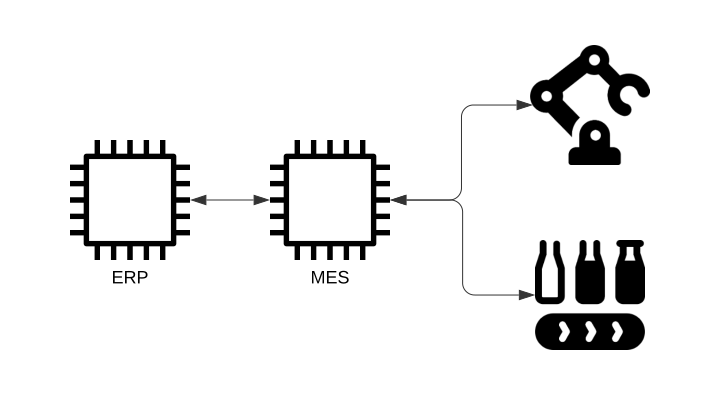
\includegraphics[scale=0.2]{images/Related/ERP.png}
    \caption{Common form of resource planning and management found in Industry 3.0 models. Source: adapted from \cite{Gilchrist2016}.}

    \label{fig:erp}
\end{figure}


The use of \acrfull{cps} allows for greater flexibility in production lines. These new systems are more responsive to factory conditions. In other words, if there is a production issue or a modification needs to be made to a particular product, the production line can respond almost instantly \cite{Gilchrist2016}. For example, if there is a missing part on a conveyor belt or a defective product, the system can quickly alert that there is a problem, and it can automatically or non-automatically take action to mitigate the consequences of that failure. This is one of the reasons why this system is more flexible. With the use of \acrfull{cps}, the \acrfull{erp} system can closely monitor the production line in real-time, giving rise to a new type of software known as \acrfull{serp}.

\begin{figure}[ht!]
    \centering
    \includegraphics[scale=0.2]{images/Related/SERP.png}
    \caption{New form of resource planning and management found in Industry 4.0 models. Source: adapted from \cite{Gilchrist2016}.}

    \label{fig:serp}
\end{figure}

The main challenges encountered in implementing Industry 4.0 are divided into two parts: management of the newly implemented technologies and technical challenges specific to each technology involved. For example, the first challenge is related to the lack of financial resources, skilled people, lack of security or understanding of the technologies. The second challenge concerns the challenges related to connectivity between technologies, e.g. communication interfaces between specific software, connectivity infrastructure, software creation challenge, complexity, etc. These two branches are the main challenges to put in place this new industry \cite{Rikalovic2022}.

\begin{figure}[ht!]
    \centering
    \includegraphics[scale=0.95]{images/Related/chalanges.png}
    \caption{The image portrays the frequency of challenges associated with the implementation of Industry 4.0 by technological areas. For the formation of this image, 47 of the 67 most relevant articles were used on technological problems in the implementation of technologies linked to this new industry model. Source: \cite{Rikalovic2022}.}

    \label{fig:chalanges}
\end{figure}

One of the challenges is the need for improved cybersecurity. The presence of multiple interconnected devices in an internal or external network raises various security concerns, as factory lines can be targets of hacker attacks, compromising the functionality of a production line or the leakage of sensitive data \cite{Gilchrist2016}. One way to mitigate security issues is the use of a Blockchain-based Authentication System (BSeIn), as proposed by the authors \textcite{LIN201842}. Additionally, another challenge is the encryption of communication between \acrfull{cps} in an industrial network. \textcite{Kreiser2018} discuss methods for creating and communicating encryption keys in a controlled environment simulating a manufacturing line. However, the implementation of security measures is limited by the available resources and the specific problem addressed.

Another challenge reported by \cite{PENAS201752} is the difficulty of integrating the virtual and physical environments. \acrfull{cps} typically employ sensors, processing units, and actuators in their operations. In addition to managing each \acrfull{cps} individually, it is necessary to understand how these units communicate with each other in a large-scale environment, enabling them to adapt to unforeseen conditions. Another problem is the lack of compatibility between real and virtual spaces, as simulations are conducted in a discrete environment, which can introduce uncertainty and imprecision \cite{Rikalovic2022}. Furthermore, the synchronization of a digital twin is a challenge for \acrfull{cps} implementation. The virtual model must be synchronized with the physical system to correctly respond to actions from the external environment. The lack of high fidelity and synchronization poses a significant challenge for the intended operation of \acrfull{cps} \cite{Zhang2017}.



Adapting existing systems to the new methodology is a significant challenge. The lack of training and skills among workers acts as a barrier to modernization, as new technologies require employees to undergo a learning curve, especially if they have been performing the same tasks for years. This can result in a substantial investment for companies, particularly small and medium-sized enterprises, and resistance to change.

Moreover, there is a need to integrate older equipment and systems with new technologies. This may involve updating obsolete components or modifying systems to ensure compatibility. Again, this can represent a considerable investment for companies, particularly small and medium-sized enterprises.

The lack of maturity of the technologies involved challenges their deployment and reliability in the industry. The authors \textcite{Rikalovic2022} report that the \acrshort{cps} do not have a widely implemented technology, few available software and communication delay issues. Not to mention that other technologies that \emph{"smart factories"} use such as: \acrfull{vr} and \acrfull{bda} aidna need to develop much more to be reliable in their employability.


In summary, these approaches to IT (Information Technology) in industry present a possible improvement of the manufacturing process. The Industrie 4.0 model is a trend that aims to promote an industrial revolution toward the use of cutting-edge technologies to increase production performance. This approach allows production lines to be more malleable both to produce products with different characteristics and to respond more quickly to unforeseen events that occur during manufacturing. In other words, it is possible for \acrshort{cps} people to make decisions autonomously or not to both unforeseen events and strategic production changes. In addition, this new industrial model brings out smart products that talk to the production line and allow information about its state to be obtained, which can help predict failures or improve customer satisfaction and have a positive impact on the product value chain \cite{economies6030046}.  However, all these technologies involved bring implementation difficulties, either due to issues involving financial resources, knowledge, security, acceptance, adaptation or maturity of the technologies.  



\section{Digital Twin}
\label{sec:digitalTwin}

The concept of Digital Twin (DT) emerged in 2003 \cite{Mihai2022, Barricelli2019} and was initially discussed by \cite{Grieves2017} in their presentation titled "Conceptual Ideal for Product Lifecycle Management" at the University of Michigan. Figure \ref{fig:digitalTwin} was included in this presentation, illustrating the key elements that would later shape the concept of DT. Although initially presented as a product management technique, it already encompassed the fundamental components that define the concept of \acrlong{dt}.

\begin{figure}[ht!]
    \centering
    \includegraphics[width=0.65\linewidth]{images/Related/CAR.pdf}
    \caption{Conceptual ideal for PLM. Dr. Michael Grieves, University of Michigan, Lurie Engineering Center, Dec 3, 2002. Adapted from: \cite{Grieves2017}.}

    \label{fig:digitalTwin}
\end{figure}

An \acrfull{dt} is a computer-based machine or model that mimics, emulates, mirrors the life of a physical entity. It continuously predicts future states and allows simulating and testing new configurations in order to preventively apply \cite{Barricelli2019} preventive maintenance operations. According to \cite{Mihai2022} such a definition corroborates with the one previously created by the authors \cite{Grieves2017}.  Indeed, the main idea behind the concept remains preserved. However, \acrshort{dt} has gained popularity in various industries and other authors have sought to evolve its definition over time, incorporating technologies such as \acrshort{ai}, machine learning, \acrshort{iot} among others. 


Grieves and Vickers  propose that the \acrfull{dt} concept consists of two systems: the physical system that has always existed and a new virtual system that contains all the information about the physical system. The virtual system is used to model and simulate the physical system in virtual space, allowing to better understand the emergent form and behaviors of the system. That is, the virtual part of the system can allow several simulations to be performed in $N$ different virtual spaces $VS_n$, in order to allow one to understand how the system behaves in these different possible environments. This helps reduce the "We didn't expect that" factor \cite{Grieves2017}.

In simple terms, a \acrfull{dt} is a system of systems. Essentially, a \acrshort{dt} is a system that enables the collection of data from different technologies and contextualizes this information in a virtual representation of an object and its interactions with other elements in its surroundings. It is a technology-based system that replicates the elements, processes, dynamics, and firmware of a physical system in a digital counterpart \cite{Mihai2022}. For example, in a case study conducted in an automotive production line in Turkey, it was collected specific data from machines and applied \acrfull{ml} techniques for data analysis \cite{Mendi2022}. This allowed simulations to be performed to identify potential issues before actual production begins, as well as provide insights on how \acrshort{dt} technology could improve efficiency and reduce downtime in that particular factory. Thus, \acrshort{dt} involves the integration of various technologies to create a virtual model that closely represents a real-world object. Figure \ref{fig:digitalTwinTree} illustrates this concept.

\begin{figure}[ht!]
    \centering
    \includegraphics[scale=0.75]{images/Related/DTTree.png}
    \caption{The Digital Twin’s central role in the Industry 4.0 era. Source: \cite{Mihai2022}.}

    \label{fig:digitalTwinTree}
\end{figure}


There are two types of \acrlong{dt}: \acrlong{dtp} and digital \acrlong{dti}. The \acrshort{dtp} describes the prototype of the physical object and contains the sets of information needed to describe and produce a prototypical physical version capable of producing a virtual version.  These information sets include fully annotated 3D Model, Bill of Materials (with material specifications), Process List, Service List, Numerical Simulations, and so on.  The \acrlong{dti} is a concept that describes a physical product that has a virtual twin attached to it for much of its life cycle. Depending on the required use cases, such a Digital Twin may contain, but is not limited to, the following sets of information: A fully annotated 3D model with sizing and geometric tolerance that describes the geometry of the physical instance and its components, a bill of materials that lists the current and all previous components, a process list that lists the operations that were performed in the creation of this physical instance along with the results of any measurements and tests on the instance, a service log that describes past services performed and components replaced, and operational states captured from actual, current, past actual and future predicted sensor data \cite{Grieves2017}. 
  

The \acrshort{dtp} model is an opportunity to identify and eliminate unforeseen and undesirable situations \cite{Grieves2017}. This type of concept allows people involved in the project to use 3D models created in \acrfull{cad} and \acrfull{cam} software, which allow them to virtually visualize and test their ideas in a simulated environment. Moreover, the use of numerical simulations such as \acrfull{fem}, \acrfull{bda} among others is also common in the design process, allowing the analysis of how the product or system will behave in different conditions and under different loads. In this way, designers can predict possible causes of failure of their product such as: failure due to structure stress, aerodynamics problems, electronic circuit design problems, communication errors between the foreseen technologies, list of required materials, etc. With this initial prototyping defined it is possible to foresee a series of failures and errors in project conception, thus avoiding unnecessary expenses with the construction of prototypes or, in the worst case, of the real product, which would not have the required performance. 

  
It is worth pointing out that \acrshort{dt} cannot be summarized simply as a software \acrshort{cad} \cite{Barricelli2019}.  For a system to be considered an \acrshort{dt}, it needs three functional blocks, these are: a physical asset, a virtual counterpart, and a communication system that allows communication between these blocks. Such a communication medium needs to be a bi-directional information flow channel that allows both output and input of data from the real model to the virtual \cite{Mihai2022}. In this way, a 3D model \acrshort{cad}, can be only one of the parts associated with building the \acrlong{dt}. 



The \acrlong{dti} allows you to understand, predict failures, and countless other possibilities about the product. This type of virtual model can have a range of information from the real product that enables the creation of virtual models that replicate physical systems, products, or assets. These are connected to their real-world counterparts via sensors and data communication networks. This enables the analysis of product histories regardless of the physical location of their counterparts. Data collected from various \acrshort{dti} can be correlated and analyzed to predict future states, helping to improve the maintenance and performance of physical systems. The ability to interrogate \acrshort{dti} provides valuable information to monitor, predict, and optimize the operations of physical systems, products, or assets. Thus, in this kind of virtual model one of the topics that is gaining prominence is preventive maintenance \cite{Grieves2017}. However, this is just one of many possibilities that this concept offers. 
  
  
Currently there are some branches of industry where there is a greater emphasis on the development of applications related to \acrshort{dt}, these sectors are: aviation, automotive, health care and predictive maintenance. The advances in these areas are due to both the potential for improvement and the importance of these areas, be it financial or human. For example, the aviation industry has a great interest in the constant monitoring of aircraft to avoid material damage or accidents with damage to human life. For the case of predictive maintenance, it can also be observed that besides the financial importance, recent technological advances allow this branch to become more and more practical. Currently, there are huge advances in developing techniques and algorithms for the prediction of possible failure points. Thus, these areas allow a great deal of practical advancement both in terms of the justification of the importance of solving potential problems and the recent availability of technologies that make this possible.  



The use of \acrshort{dt} in manufacturing can provide an improvement in process efficiency through task automation and in supporting decision making \cite{ROSEN2015567}. \textcite{Qi2018} also report that the use of \acrfull{bd} allows \acrshort{dt} to achieve improved process efficiency and predictions on data collected along the manufacturing line. For example, the use of \acrshort{bda} allows the attempt to predict possible failure points both throughout the life of a product and the occurrence of failures in machinery involved in its manufacture, figure \ref{fig:digitalTwinBigData}. In this way, \acrshort{bda} has great potential for use in predictive maintenance or for adapting the product to certain standards that satisfy the interests of the end user. \textcite{Tao2017} explore the idea of using \acrshort{dt} for the shop floor of a production line through ways of implementing the concept. That is, methods of implementing a virtual counterpart of the production line. This way, possible points of failure can be analyzed and layout or process optimizations applied. In this way, \acrshort{dt} is currently being used more and more in factories to improve processes and products.

In the aeronautical industry, the use of \acrshort{dt} is used more for the predictive area, that is, to detect the appearance of possible failure points and trigger mitigation systems \cite{Barricelli2019}. By means of statistical methods and with numerical approaches involving multi-physics systems it is possible to estimate possible aircraft failures through initial input data \cite{Benjamin2012}. An example is the case in which \textcite{Bielefeldt2015} propose the use of \acrlong{fem} with \acrshort{dt} to obtain possible failure points on a wing of a commercial aircraft. Thus, currently, the use of \acrshort{dt} has an important role in predicting possible unforeseen events or failures that may occur in an aircraft, which can cause enormous damage to property and human life. With the presence of a system that can previously detect possible errors it is possible to mitigate these occurrences or solve them with correction and safety strategies or techniques. 

\begin{figure}[ht!]
    \centering
    \includegraphics[scale=0.75]{images/Related/cps.png}
    \caption{Information of the life cycle of a product through the use of cybernetic physical systems. Source: \cite{Qi2018}.}

    \label{fig:digitalTwinBigData}
\end{figure}

Recently, the area of medical care is another branch that has been achieving great advances in the implementation of new technologies and techniques. \acrlong{dt} is one of the new concepts being implemented in the healthcare area with the goal of creating a virtual system of the human body or its organs in order to achieve the goal of predicting possible diseases or malfunctions of the human body, as well as managing the availability of assets in a hospital. The \textcite{johns_2016} made use of \acrshort{ann} to perform simulations and make the best possible decisions for managing its resources, which is crucial for saving lives. Another case was the use of a \acrshort{dt} by Siemens Healthineers at Mater Private Hospitals (MPH) in Dublin \cite{gilligan_digital_2018}. In this case study, the hospital had a lack of space, beds, delays, and high patient demand. To solve these problems, Siemens Healthineers redesigned the radiology department with the development of a \acrshort{ann} to manage the department and its operations. With this, a \acrshort{dt} of the department was obtained, allowing simulations to be performed to find an optimal layout and control and monitoring of tasks. Another example of \acrfull{dt} is the \emph{The Living Heart} \cite{Levine2022}, Figure \ref{fig:digitalTwinHeart}, this project allows scientists to simulate the human heart. It allows a realistic, multi-phase simulation to be performed, which takes in various physical fields such as electromagnetic, fluid dynamics, and mechanics. In this way, scientists can use this tool to aid studies of how certain physical stresses or cardiovascular diseases may impact the functioning of this organ. 

\begin{figure}[ht!]
    \centering
    \includegraphics[scale=0.65]{images/Related/heart.png}
    \caption{Stresses  simulation depicted on a 3D rendering of the Living Heart Model. Source: \cite{Levine2022}.}

    \label{fig:digitalTwinHeart}
\end{figure}


In summary, the concept of \acrfull{dt} has remained quite stable since its creation in 2002, undergoing adaptations to the technological changes that have been appearing. The \acrshort{dt} is formed by two parts: the physical system and the virtual system. The function of the \acrshort{dt} is to contextualize data from different technologies into a virtual representation of an object and how it interacts with its surroundings. In this way, various technologies can be integrated into this system such as: \acrlong{ann}, \acrlong{bda}, \acrlong{iot}, \acrlong{vr}, \acrlong{vr} among others. With this data generated and processed, it is possible to obtain data about: possible future failures, location information, current physical state, end user interests about the product, etc. In general, \acrshort{dt} is part of the new industrial revolution with enormous potential to reduce costs and increase the productivity of production lines, besides enabling the final product to have a longer life and be safer. 
\section{Review of current traceability systems in the  industry}\label{section: woodFurnitureIndustryTraceabilityReview}

Currently, traceability is employed in several productive sectors, presenting a wide range of applications. Among them are the implementation of \acrfull{mcp} \cite{ZHONG2013}, stock controls \cite{Anssens2011, Yue2011}, production control \cite{Engelhardt2012}, counterfeit prevention \cite{Rida2007}, among other possibilities. The use of a traceability system can significantly improve the execution of tasks in a factory, allowing not only greater control of inventory, but also of the processes themselves. By identifying critical points in production, it is possible to implement actions to mitigate their occurrence and, consequently, make processes more efficient \cite{Chua2012}.


Nonetheless, the comprehension of the traceability concept is indispensable. As per the ISO 9000:2015 standard \cite{iso_9000_2015}, traceability is characterized as the "capacity to trace the history, application, or location of that which is under consideration." To elucidate, within the confines of a production line, traceability denotes the competency to procure an exhaustive historical record pertinent to the product or process. Diverse mediums may be employed for the storage of this information, ranging from paper-based systems to electronic or semi-electronic methodologies.

Subsequently, it is plausible to contemplate the implementation of a hybrid system. Such an approach amalgamates the utilization of conventional paper-based systems with the deployment of digital technologies. This synergy augments the performance metrics associated with tracing products, processes, and the archival of production and inventory records \cite{Qu2012-hw, ZHONG2013, Gilchrist2016}. The architecture of a hybrid system encompasses an assortment of components, including but not limited to printed documents, spreadsheets, manual entries, Enterprise Resource Planning (ERP), and Manufacturing Execution Systems (MES).


However, the hybrid system faces challenges in achieving real-time traceability. One possibility to overcome these obstacles is to incorporate \acrfull{iot} and \acrshort{m2m} communication components, enabling a real-time connection to the \acrshort{erp} or allowing decision making without the intervention of an intermediary agent. The integration of advanced technologies can significantly enhance the efficiency and adaptability of the hybrid system, contributing to greater flexibility and accuracy in the traceability of industrial processes \cite{Gilchrist2016}.

\subsection{Use of RFID for traceability}\label{RFIDtraceability}

The implementation of \acrfull{rfid} sensors is vastly employed in the traceability of components in industry, with applications in various \cite{ZHONG2013, Qu2012-hw, Anssens2011, Engelhardt2012, Rida2007} sectors. The initial concept of RFID dates back to Harry Stockman's paper entitled "Communication by Means of Reflected Power," published in 1948. The idea demonstrated great relevance in aircraft identification by the military sector, especially due to the advances in radar development that occurred during World War II \cite{Landt2005}. This technological innovation allowed for significant improvements in tracking efficiency and accuracy, paving the way for broader industrial and commercial applications in the future.

However, the implementation of RFID technology requires a specific infrastructure, the feasibility of which can vary depending on the added value provided by its use. For the RFID system to function properly, some fundamental components are necessary, such as: an antenna, a transceiver, middle-ware software, a database, and a transponder \cite{MCFARLANE2003365}. Figure \ref{fig:rfid} illustrates the typical configuration of an RFID system.

\begin{figure}[h!]
    \centering
    \includegraphics[width=.65\linewidth]{images/Development/chap3/g1126.png}
        \caption{Simple schematic of an Auto ID system. Source: \cite{MCFARLANE2003365}}

    \label{fig:rfid}
\end{figure}

In this context, the analysis of the feasibility of adopting \acrshort{rfid} technology should consider the costs and benefits associated with its implementation. The necessary infrastructure might represent a significant investment, which should be justified by the expected return in terms of operational efficiency, error reduction, and optimization of the involved processes. Therefore, the decision to adopt \acrshort{rfid} technology should be based on a thorough evaluation of the specific needs of each application and the value it can effectively add.


The selection of technologies to be used in the \acrshort{rfid} system has direct implications on the costs associated with its implementation. There are three categories of \acrshort{rfid} tags available on the market: passive, active, and battery-assisted passive. Each type has distinct characteristics, which influence both the performance and costs of the system. Among the three options, passive tags are the most economical. These tags do not have an internal battery and, consequently, are powered by the energy transmitted by the reader's antenna. Despite being more financially accessible, passive tags have a limited range and can be affected by interference caused by metallic materials and liquids in the environment. On the other hand, active and battery-assisted passive tags, although more costly, offer a greater range and higher resilience to interference \cite{Lee2012}. The choice between these types of tags should take into account the specificity of the application, such as the need for a greater range or tolerance to interference, as well as the availability of financial resources for investment in the \acrshort{rfid} system infrastructure.


The feasibility analysis for the implementation of an inventory management system using \acrshort{rfid} technology is a complex task, as it requires the weighing of multiple factors, such as the predictability of inventory flow, fixed costs, and especially, the technologies involved in the process. Several studies have been conducted to assess the financial feasibility of using \acrshort{rfid} in different contexts.

\textcite{Yue2011}, for example, conducted a simulation of the feasibility of using \acrshort{rfid} in a pharmaceutical supply chain. The authors concluded that, using the \acrfull{npv} method, the venture might not be viable. Therefore, they suggested using the \acrfull{rov} method for a more accurate analysis.

In contrast, \textcite{Ustundag2007} conducted a case study in a parcel delivery company and found that the venture is viable, although the return time varies according to the type of \acrshort{rfid} tag chosen. It is worth noting that this case study does not provide detailed information.

Finally, \textcite{Lee2012} presented an improved methodology for the financial evaluation of investment in radio frequency identification systems. In this paper, the authors introduce a mathematical model capable of quantifying the feasibility of the venture, taking into account inventory flow, fixed costs, and \acrfull{jit} or \acrfull{eoq} inventory models. In this model, the authors address three main aspects:

\begin{enumerate}
  \item Investment in order efficiency;
  \item Investment in JIT efficiency;
  \item Simultaneous investment decisions in \acrfull{rfid}.
\end{enumerate}

The mathematical model proposed by \textcite{Lee2012} is composed of four cost components: ordering cost during a planning period ($\frac{OD}{Q^{*}}$), the efficiency factor of the process tied to \acrshort{rfid} technology (R), inventory holding cost ($ \frac{HQ^*}{2} $), \acrshort{jit} efficiency (I), order efficiency investment cost (K), and \acrshort{jit} efficiency investment cost (V). 

 In this model, the authors address three main aspects, one of which is \acrshort{jit} efficiency, which is defined as the degree to which the time interval between the delivery point and the consumption/production time is reduced by investment V.


However, for the case of the company that is the subject of the current work, the inventory flow is much smaller compared to the three previously analyzed works, in addition to involving products that may not have such a high added value. For this reason, the adoption of the RFID system may not be a plausible approach.

\subsection{Use of QR Code for traceability}\label{QRtraceability}

The QR code, conceived by Toyota subsidiary Denso Wave in 1994, was established with the purpose of facilitating the tracking of automotive components. The motivation behind the development of the QR code resided in the limitation of the information capacity of traditional bar-codes, which can only accommodate 20 alphanumeric characters. This technological innovation proved its efficiency by providing greater control and accuracy in tracking the parts used in the automotive industry \cite{Tiwari2016}.

Over time, the application of the QR code expanded to various other sectors, establishing itself as a valuable tool for enhancing traceability, inventory management, commercial applications, event ticketing, electronic transactions, and other relevant functionalities \cite{Tiwari2016}.

The operation of the QR code system is based on two main components that work together to encode and decode information: the QR code encoder and the decoder. The encoder is responsible for processing the data and generating the QR Code, while the decoder extracts and interprets the data stored in the QR code, see figure \ref{fig:qr}. The structure of the QR Code is formed by modules, which are the black and white dots that make up the code. These modules are organized into symbols ranging from Version 1 to Version 40, each with a distinct configuration of modules, starting with Version 1, which contains 21 × 21 modules, up to Version 40, with 177 × 177 modules \cite{iso_18004_2015}. This organization allows for the efficient encoding and decoding of information, ensuring the effectiveness of the QR Code as a tool for traceability and data storage in various contexts and applications \cite{Tiwari2016}.


\begin{figure}[h!]
\centering
\includegraphics[width=.65\linewidth]{images/Development/chap3/QR.pdf}
\caption{Working (overview) of QR Code. Adapted from: \cite{Tiwari2016}}
\label{fig:qr}
\end{figure}

Despite the numerous advantages of QR Code over barcode, especially in terms of speed and data storage capacity, the QR Code still has capacity limitations. Each version of the QR symbol has a maximum data capacity, which depends on the amount of data, the type of character, and the error correction level \cite{Tiwari2016}. In other words, as the amount of data increases, more modules are needed to compose the QR Code, resulting in a larger QR Code symbol, see table \ref{tab:qrcode-capacity}. Therefore, although the QR Code offers significant benefits in terms of traceability and information storage, it is important to consider its capacity limitations when selecting the best solution for a given context or application.

\begin{table}[!ht]
\begin{tabular}{llllllll}
\hline
\multicolumn{8}{c}{DATA CAPACITY OF QR CODE VERSION 40 } \\
\cline{1-8}

Version             & Modules                  & ECC Level & Data Bits & Numeric & Alphanumeric & Binary & Kanji \\
\cline{1-8}


\multirow{4}{*}{40} & \multirow{4}{*}{177x177} & L         & 23,648    & 7,089   & 4,296        & 2,953 & 1,817 \\
                    &                          & M         & 18,672    & 5,596   & 3,391        & 2,331 & 1,435 \\
                    &                          & Q         & 13,328    & 3,993   & 2,42         & 1,663 & 1,024 \\
                    &                          & H         & 10,208    & 3,057   & 1,852        & 1,273 & 784 \\
\cline{1-8}
\end{tabular}
\caption{QR Code Capacity. Adapted from: \cite{Tiwari2016}}
\label{tab:qrcode-capacity}
\end{table}

In conclusion, the QR code, initially designed to optimize the tracking of automotive components, has experienced a remarkable evolution since its creation, establishing itself as a multi-functional and comprehensive tool, applicable in various sectors. The ability to store information efficiently, coupled with the ease of use through mobile devices and comparatively lower cost compared to other solutions such as Radio Frequency Identification (RFID), gives the QR code a valuable solution in improving traceability and data management in various contexts. However, it is crucial to consider the inherent limitations of the QR code's capacity when selecting the most suitable alternative to meet specific demands for tracking and information storage. In this sense, the QR code persists as a technological innovation of relevance, capable of providing significant contributions to the efficiency and effectiveness of traceability processes, as well as to the storage and sharing of information in different environments, within its limitations.

\section{State of the Art in Traceability for Wood Work}\label{section:stateOfArt}
One of the driving forces behind the development of this work is the noticeable scarcity of research and solutions addressing the traceability of the wood fabrication process. In the academic circle, a limited number of existing solutions are being explored and studied. Indeed, only a handful of scientific articles that delve into this topic were identified. The majority of the available literature predominantly concentrates on supply chain aspects and employs technologies such as Radio Frequency Identification (RFID),  block-chain, QR Code, Fingerprint Methods, that can be utilized to address the identification of timber logs.

The employment of Radio Frequency Identification (RFID) technology offers substantial advantages for real-time tracking in the wood supply chain. However, its feasibility hinges on an in-depth financial analysis concerning the impact of implementation \cite{Ustundag2007}. \textcite{Lee2012} present a methodological and comprehensive analysis in their article, which considers the substantial initial investments required for the deployment of this technology. In conclusion, the feasibility of adopting RFID technology will depend on the scale of application and the specific aspects that the technology aims to address, as well as the inventory model that will be employed, whether it be \acrfull{jit} or \acrfull{eoq}.

In their study, \textcite{hultgren2018blockchain} present an approach employing block-chain technology for the traceability of the supply chain in the timber production process. Furthermore, their approach facilitates the integration of additional stages into this block-chain model. However, it's important to note that the model does not support real-time monitoring of the traceability. To achieve real-time tracking, the incorporation of supplementary technologies would be necessary. Block-chain, in this context, offers transparency and security, but for more dynamic tracking, complementary tools and technologies need to be considered.

In another case study conducted by  \textcite{Amaya2022}, a system based on a web solution coupled with QR Codes was utilized for the tracking of timber logs. The system developed by the authors essentially allows IoT devices or users to input data into the system which can then be accessed and monitored through a web platform. Moreover, in order to facilitate easy tracing of timber logs in the cutting and extraction environment, QR Codes are attached to the logs. When scanned, these QR Codes redirect the user to the web application, providing a historical record of information pertaining to that specific log. This approach combines the accessibility of web platforms with the ease of QR Code technology, creating an efficient and user-friendly tracking system for timber management.

In a scholarly article authored by  \textcite{Schraml2020}, an attempt is made to establish a fingerprinting standard for timber logs. The authors have developed a methodology which employs spectral scanning systems to acquire detailed hyperspectral data (HSD) of timber. Subsequently, high-resolution images are captured and processed through computer vision techniques for the segmentation of individual timber pieces. Through this approach, the authors manage to extract detailed information about each timber log, effectively characterizing each log with unique features. In a parallel development, \textcite{Sun2021} also utilize a computer vision-based approach for deriving fingerprints of timber logs, but through a pure \acrfull{cnn} approach. In their methodology, the authors employ the AKAZE computer vision technique to identify wood grain patterns for each timber log, which can then be used to uniquely identify them. Both these studies highlight the innovative use of computer vision and spectral analysis techniques in establishing unique identifiers for timber logs, which can have significant implications for traceability and management in the wood work industry.

% \subsection{Use of Artifical Inteligency in traceability}\label{ArtificialIntelligencetraceability}

% The use of barcodes and RFID is a widely adopted practice in product tracking, both in production and in stock. However, these methods present some limitations. The use of barcodes, for instance, has a restricted capacity for information storage and can be easily damaged, which hampers reading. Additionally, the employment of RFID also faces the issue of potential damages, besides the high costs associated with the infrastructure required for its operation \cite{Pihir2011}.  \textcite{Elisabeth2011} also mention the difficulties of using RFID for certain types of materials that can interfere with the reading of radio waves, which may demand more robust tags and further increase the involved costs.

% Over the past few years, the exponential growth of e-commerce has driven significant advancements in goods warehousing management, due to the increase in the scale and complexity of operations involved in this scope. Currently, companies are employing a broad range of advanced technologies, such as QR codes, machine vision systems, communication modules, microcomputers, servers, and RFID, which allow the integration of sophisticated systems that apply artificial intelligence in strategic decision-making. This technological evolution has proven to be crucial in improving storage management and optimizing the efficiency and effectiveness of operations, meeting the growing demands and challenges imposed by the constantly expanding e-commerce \cite{Hristov2022}.

% The application of artificial intelligence in traceability processes transcends decision-making in the industrial context. For example, \textcite{Hristov2022} employed \acrfull{cnn} in object detection, enabling robots to identify items in a storage center and, consequently, speeding up decision-making in performing their tasks. This innovative approach demonstrates the potential of artificial intelligence to enhance the efficiency and precision of traceability processes, as well as allowing for inventory traceability, contributing to greater adaptability and dynamism in the operations of storage and movement of goods.

% In contrast to traditional item tracking methods,  \textcite{Patel2020} propose an innovative approach using \acrshort{cnn}, specifically with the ResNet-50 architecture. In this methodology, they employed transfer learning techniques to enable agile adaptation of the data model in scenarios with a limited amount of training images. Consequently, they achieved an image tracking rate of 4 \acrfull{fps}, considering the adopted software and hardware settings, enabling real-time object traceability.

% Another important aspect to be considered is the possibility of customizing \acrshort{cnn}s to meet the specific needs of different industries and sectors. Through the use of appropriate architectures and algorithms, it is possible to develop tracking solutions adapted to the particularities of each scenario, optimizing the efficiency and effectiveness of operations.


